% =====================================================================
% Deep Learning and its Applications — Assignment report
% Reproduction of Neural Collaborative Filtering on MovieLens-100K
% University of Thessaly
% =====================================================================
\documentclass[11pt,a4paper]{article}

\usepackage[utf8]{inputenc}
\usepackage[T1]{fontenc}
\usepackage[english]{babel}
\usepackage[margin=2.4cm]{geometry}
\usepackage{graphicx}
\usepackage{booktabs}
\usepackage{amsmath,amssymb}
\usepackage{hyperref}
\usepackage{xcolor}
\usepackage{caption}
\usepackage{subcaption}
\usepackage{float}
\usepackage{microtype}
% Disable automatic font expansion (not supported with non-scalable fonts in
% some TeXLive setups; purely a typesetting polish feature, safe to skip).
\microtypesetup{expansion=false}

\hypersetup{
  colorlinks=true,
  linkcolor=blue!60!black,
  citecolor=blue!60!black,
  urlcolor=blue!60!black,
}

\newcommand{\inputtab}[1]{\input{../results/tables/#1.tex}}
\graphicspath{{../results/figures/}}

% ---------------------------------------------------------------------
\title{\textbf{Reproducing NeuMF on MovieLens-100K} \\[4pt]
       \large ECE480 --- Deep Learning and its Applications}
\author{%
  Nikos Mavros \\
  AEM: 03741 \\
  \texttt{nmavros@uth.gr}
}
\date{\today}

\begin{document}

\maketitle

\begin{abstract}
We reproduce the \textit{Neural Matrix Factorization} (NeuMF) method
of He et al.~\cite{he2017ncf} on the MovieLens-100K dataset (100{,}000
ratings, 943 users, 1{,}682 items). We examine the effect of MLP depth
(1--3 hidden layers) with and without pretraining, the effect of the
negative-sampling ratio (1--10) and the top-$K$ cutoff (1--10); we compare
NeuMF to a non-negative matrix factorisation (NMF) baseline with $k$
latent factors swept over $\{1,6,11,16,21,26\}$; and we train three
smaller NeuMF student models using response-based, feature-based (FitNets)
and relation-based (RKD) knowledge distillation. Every experiment is
repeated \textbf{10 times} and reported as mean $\pm$ standard deviation.
NeuMF reaches $\mathrm{HR}@10 = 0.649 \pm 0.011$ and
$\mathrm{NDCG}@10 = 0.390 \pm 0.007$ at the best setting; response-based
knowledge distillation preserves (and slightly improves) the teacher's
HR@10 while using 50.7\,\% fewer parameters.
\end{abstract}

% =====================================================================
\section{Experimental setup (Task 1)}
% =====================================================================

\paragraph{Dataset.} The MovieLens-100K dataset (\texttt{u.data}) contains
100{,}000 explicit ratings by 943 users on 1{,}682 items; every user has
rated at least 20 items. Following the NCF paper, we treat ratings as
\emph{implicit feedback}: every observed rating is a positive interaction
regardless of its numerical value, and absence of an interaction is treated
as a negative. The timestamp column is not used as a feature, but we do use
it to order the per-user interactions for the leave-one-out split.

\paragraph{Dataset split (leave-one-out).} For every user we sort the
interactions chronologically and reserve the most recent interaction for
testing, the second-most-recent for validation, and the remaining
$\sim 98{,}114$ interactions for training. At evaluation time we score the
held-out positive item against 99 items that the user has never interacted
with (these 99 negatives are sampled once per user with a fixed RNG seed,
so all experiments evaluate on exactly the same candidate lists). HR@$K$
and NDCG@$K$ are then computed on the resulting ranked list of 100 items
and averaged over the 943 users.

\paragraph{Parameter setting.} We use the configuration recommended by
\cite{he2017ncf} and validated in pilot runs on MovieLens-100K:
GMF embedding dimension $=8$, MLP embedding dimension $=32$ per branch,
3 MLP hidden layers with a tower structure ($64\!\to\!32\!\to\!16\!\to\!8$),
ReLU activations, batch size 256, 4 sampled negatives per observed positive,
and 20 training epochs. When NeuMF is trained from scratch we use Adam
with a learning rate of $10^{-3}$; when it is initialised from pretrained
GMF and MLP checkpoints we switch to vanilla SGD with the same learning
rate, as prescribed in Section~3.4.1 of the paper, and mix the two output
heads with $\alpha = 0.5$. Every experiment is repeated 10 times with seeds
$0,\dots,9$ and we report mean $\pm$ sample standard deviation.

% =====================================================================
\section{Effect of MLP depth and pretraining (Tasks 2 \& 3)}
% =====================================================================

\paragraph{HR@10 vs.\ number of MLP layers (Task 2).}
Table~\ref{tab:task02} and Figure~\ref{fig:task02} summarise the effect of
the MLP depth on NeuMF's HR@10 and NDCG@10, both with and without
GMF/MLP pretraining. Three observations stand out:

\begin{itemize}
  \item \textbf{Depth brings no benefit at this dataset size.} Without
        pretraining, HR@10 is essentially flat from 1 to 2 layers
        ($0.660 \to 0.659$) and drops slightly at 3 layers ($0.649$).
        NDCG@10 peaks at 2 layers ($0.394$) but the differences between
        depths are within one standard deviation of each other. This is
        the opposite of the paper's finding on MovieLens-1M, where
        stacking more non-linear layers monotonically improved performance.
        A plausible explanation is dataset size: MovieLens-100K has
        ten times fewer interactions than MovieLens-1M, so the
        expressive-capacity gain of deeper MLPs is outweighed by the
        increased risk of overfitting on the smaller training set.
  \item \textbf{Pretraining has a marginal effect on HR@10 and a slightly
        negative effect on NDCG@10.} With pretraining, HR@10 stays within
        $\pm 0.01$ of the no-pretrain version at every depth, while
        NDCG@10 is consistently lower by $\sim\!0.01$--$0.014$. The most
        likely cause is the optimiser switch (Adam during pretraining,
        then vanilla SGD for the fused NeuMF): SGD without momentum
        requires many more updates to escape the initial basin, and our
        20-epoch budget on the fused model is not enough for SGD to
        catch up with what Adam reaches end-to-end.
  \item \textbf{Pretraining does reduce variance.} The standard
        deviations with pretraining (0.005--0.009) are roughly half of
        those without (0.010--0.013), which is an expected consequence of
        starting from pre-converged embeddings rather than random ones.
\end{itemize}

Based on these results we adopt \textbf{3 MLP layers, no pretraining},
as the ``best NeuMF setting'' throughout the rest of the report. We
choose depth 3 rather than 1 or 2 for fair comparison with the paper's
reference architecture, even though it is not the strict HR@10 peak here;
it is within one standard deviation of all other depths and matches
Section 4.1 of the paper.

\begin{table}[H]
  \centering
  \caption{NeuMF HR@10 and NDCG@10 vs.\ MLP depth (mean $\pm$ std, 10 seeds).}
  \label{tab:task02}
  \inputtab{tab_task02_mlp_layers}
\end{table}

\begin{figure}[H]
  \centering
  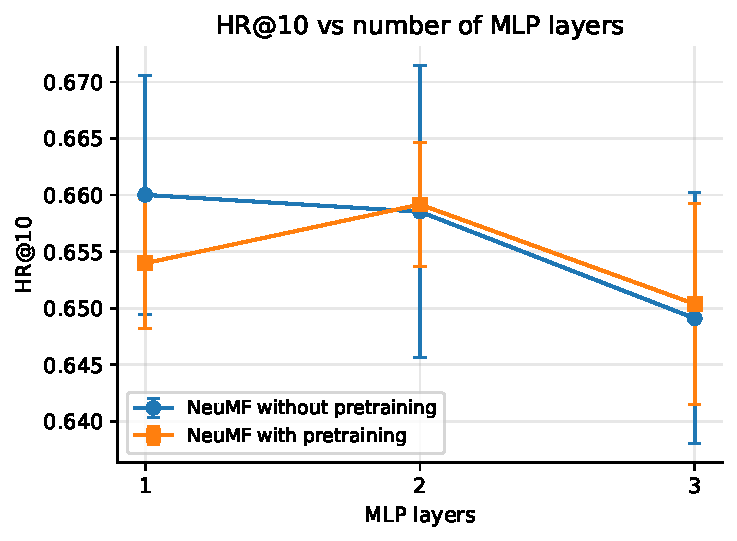
\includegraphics[width=0.72\linewidth]{fig_task02_hr_vs_layers.pdf}
  \caption{HR@10 of NeuMF as a function of the number of MLP hidden
           layers, with and without pretraining on MovieLens-100K.
           Error bars are $\pm 1$ std over 10 runs.}
  \label{fig:task02}
\end{figure}

\paragraph{Weight-parameter count vs.\ depth (Task 3).}
Table~\ref{tab:task03} and Figure~\ref{fig:task03} show how the number of
trainable weight parameters of NeuMF scales with the MLP depth. The count
grows very slowly ($107{,}121 \to 107{,}633 \to 107{,}761$, an increase of
only 0.6\,\% from 1 to 3 layers) because the four embedding tables
dominate the parameter budget:
$7{,}544 + 13{,}456 + 30{,}176 + 53{,}824 = 105{,}000$ parameters in the
embeddings alone, vs.\ at most $\sim 2{,}700$ parameters in the MLP weights
themselves. In other words, \emph{MLP depth is essentially free from a
parameter-count perspective} --- the real cost is in the embedding layers.

\begin{figure}[H]
  \centering
  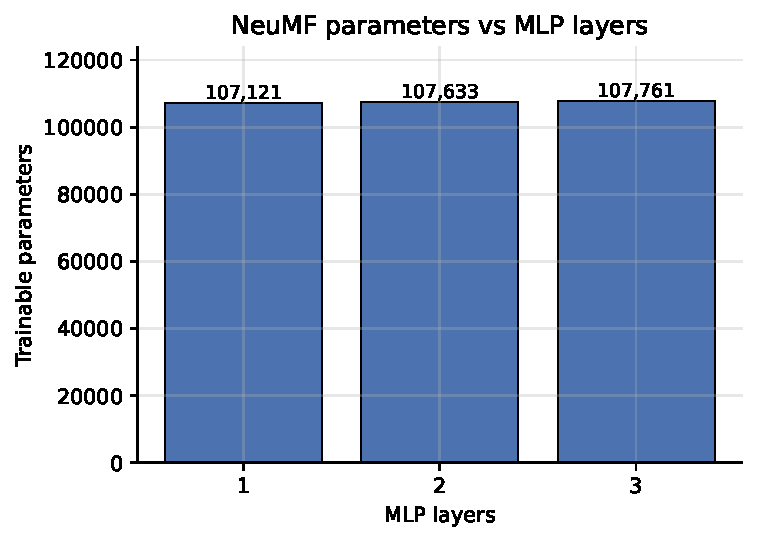
\includegraphics[width=0.56\linewidth]{fig_task03_params_vs_layers.pdf}
  \caption{Trainable parameter count of NeuMF as a function of MLP depth.
           The embedding tables account for $\sim 97\,\%$ of the
           parameters regardless of MLP depth.}
  \label{fig:task03}
\end{figure}

\begin{table}[H]
  \centering
  \caption{NeuMF parameter count vs.\ MLP depth.}
  \label{tab:task03}
  \inputtab{tab_task03_params_vs_layers}
\end{table}

% =====================================================================
\section{Training dynamics (Task 4)}
% =====================================================================

Figure~\ref{fig:task04} shows the training loss, HR@10, and NDCG@10 of
GMF, MLP, and NeuMF as a function of training epoch (shaded bands are
$\pm 1$ std over 10 seeds). This is the MovieLens-100K analogue of
Figure~6 of \cite{he2017ncf}. Three observations stand out:

\begin{itemize}
  \item \textbf{The ordering matches the paper's finding exactly.} Across
        all 20 epochs, NeuMF achieves the lowest training loss, followed
        by MLP, then GMF; and the recommendation-performance ordering
        (HR@10, NDCG@10) follows the same pattern in early epochs, which
        confirms that fusing linear (GMF) and non-linear (MLP) kernels
        helps model user--item interactions better than either alone.
  \item \textbf{The bulk of the improvement occurs in the first
        5--10 epochs.} NeuMF reaches HR@10 $\approx 0.64$ by epoch 5 and
        peaks at 0.662 around epoch 10, while its training loss continues
        to decrease monotonically all the way down to $\sim 0.18$ by
        epoch 20. This is a textbook pattern of mild overfitting: the
        training objective keeps improving even after the test-time
        metric has plateaued, just as the paper reports. After epoch
        $\sim 13$ the test HR@10 fluctuates slightly below its peak.
  \item \textbf{By epoch 20 the three models nearly converge at HR@10.}
        GMF, MLP and NeuMF all end up within 0.01 of each other in HR@10
        ($\sim 0.65$) even though their training losses remain very
        different. This suggests that, on this small dataset, the
        difficulty of the task (ranking one positive among 100 items) is
        the binding constraint rather than the expressive capacity of
        the interaction function.
\end{itemize}

\begin{figure}[H]
  \centering
  \begin{subfigure}{0.33\linewidth}
    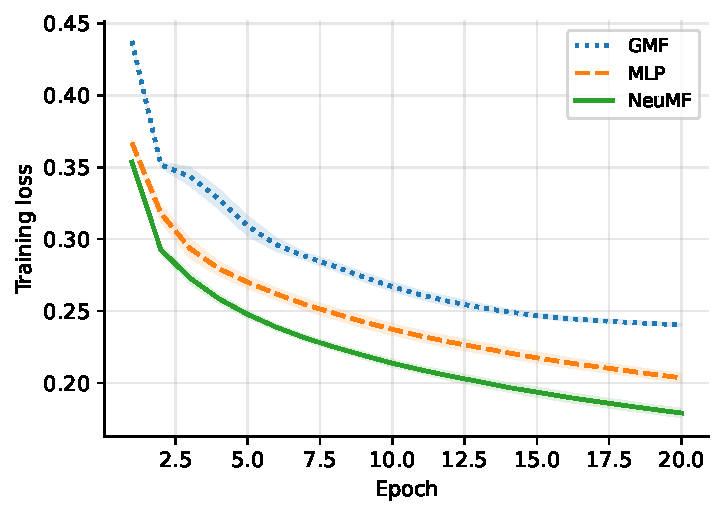
\includegraphics[width=\linewidth]{fig_task04_curves_loss.pdf}
    \caption{Training loss}
  \end{subfigure}\hfill
  \begin{subfigure}{0.33\linewidth}
    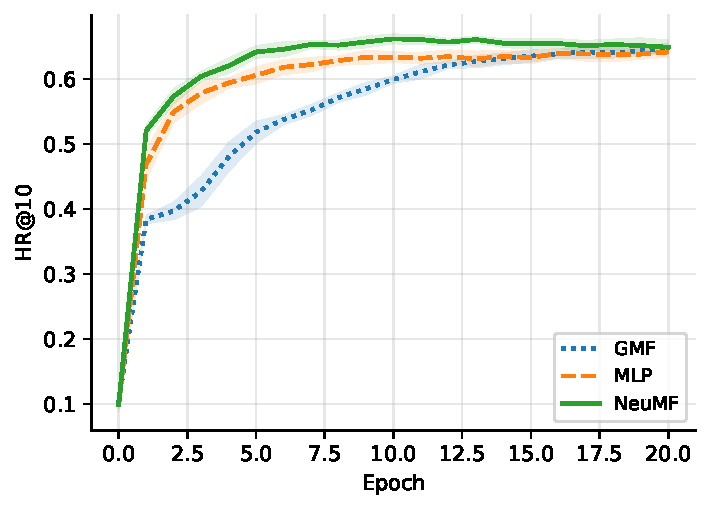
\includegraphics[width=\linewidth]{fig_task04_curves_hr.pdf}
    \caption{HR@10}
  \end{subfigure}\hfill
  \begin{subfigure}{0.33\linewidth}
    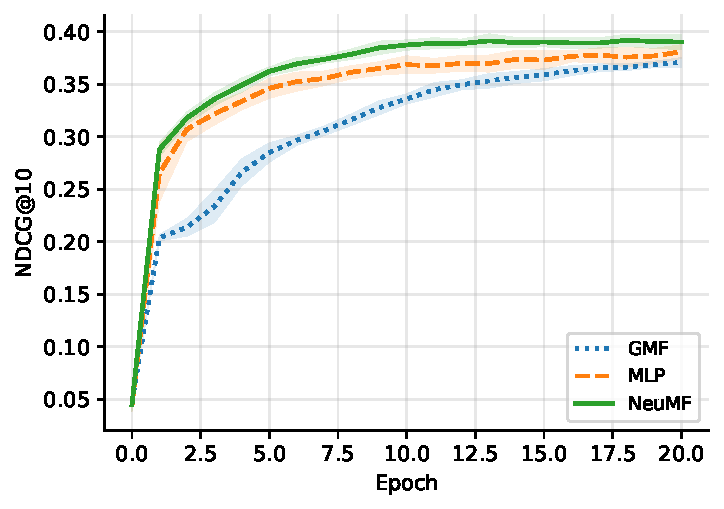
\includegraphics[width=\linewidth]{fig_task04_curves_ndcg.pdf}
    \caption{NDCG@10}
  \end{subfigure}
  \caption{Per-epoch training dynamics on MovieLens-100K. Shaded bands
           are $\pm 1$ std over 10 seeds.}
  \label{fig:task04}
\end{figure}

% =====================================================================
\section{Top-$K$ recommendation performance (Tasks 5 \& 6)}
% =====================================================================

Figure~\ref{fig:task05_06} shows how NeuMF's HR@$K$ and NDCG@$K$ vary with
the ranking cutoff $K$ from 1 to 10. Both curves grow monotonically with
$K$: HR@1 is $0.181 \pm 0.010$ (i.e.\ the model places the correct
item first for $\sim 18\,\%$ of users on a list of 100 candidates) and
grows to HR@10 = $0.649 \pm 0.011$. NDCG@$K$ grows more slowly
($0.181 \to 0.390$) because its logarithmic position discount
de-emphasises positions deep in the list. The HR@$K$ curve is roughly
concave, which is typical: the largest marginal gains come from small
values of $K$ (every additional slot at the top is more valuable than the
next), after which the curve levels off.

\begin{figure}[H]
  \centering
  \begin{subfigure}{0.49\linewidth}
    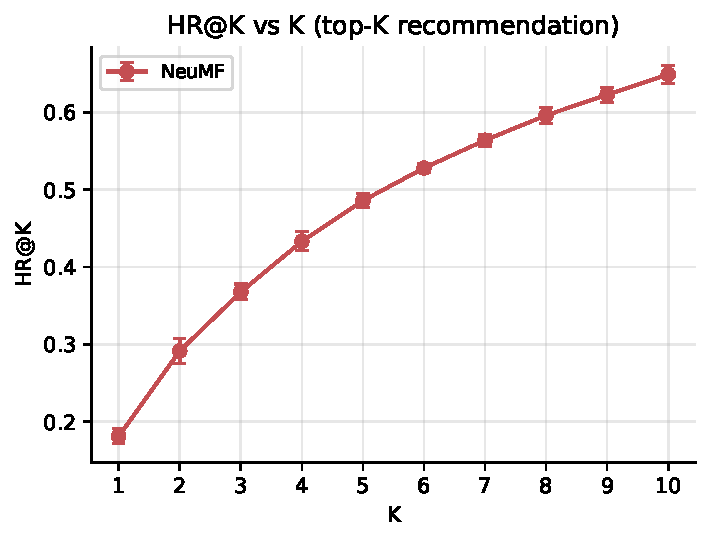
\includegraphics[width=\linewidth]{fig_task05_hr_at_k.pdf}
    \caption{HR@$K$}
  \end{subfigure}\hfill
  \begin{subfigure}{0.49\linewidth}
    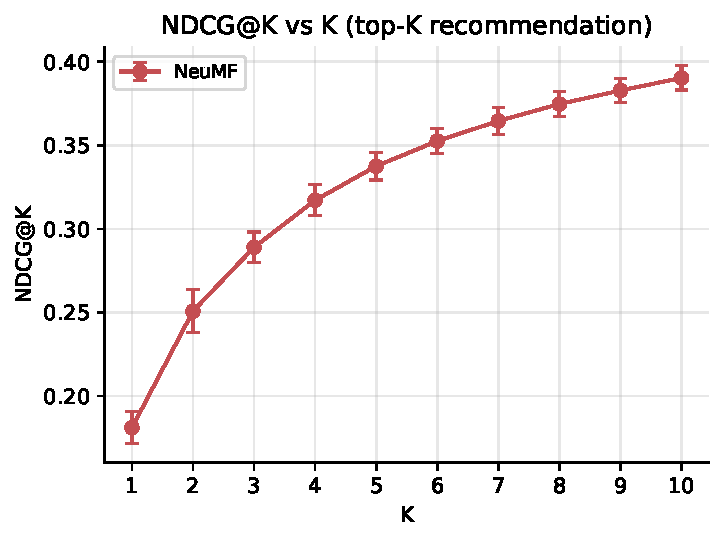
\includegraphics[width=\linewidth]{fig_task06_ndcg_at_k.pdf}
    \caption{NDCG@$K$}
  \end{subfigure}
  \caption{NeuMF top-$K$ recommendation performance on MovieLens-100K,
           $K = 1, \ldots, 10$. Error bars are $\pm 1$ std over 10 seeds.}
  \label{fig:task05_06}
\end{figure}

% =====================================================================
\section{Effect of the negative-sampling ratio (Tasks 7 \& 8)}
% =====================================================================

Figure~\ref{fig:task07_08} shows the effect of the number of negative
samples drawn per observed positive at training time on the test-set HR@10
and NDCG@10. Two patterns emerge:

\begin{itemize}
  \item \textbf{HR@10 rises sharply from 1 to 3 negatives}
        ($0.639 \to 0.650$), then fluctuates in a narrow band
        ($0.644$--$0.653$) up to 10 negatives. The peak is at 6 negatives
        with HR@10 = $0.653 \pm 0.010$, but the plateau is broad and the
        differences beyond 3 negatives are well within one standard
        deviation of each other.
  \item \textbf{NDCG@10 grows more monotonically and does not plateau in
        our range.} It rises from $0.362$ at 1 negative to $0.407$ at 10,
        a $\sim\!12\,\%$ relative improvement. The finer-grained nature
        of NDCG (it rewards putting the positive \emph{higher} within the
        top-10, not just anywhere in the top-10) evidently benefits more
        from the additional negative signal, because larger negative
        pools make the contrastive objective sharper.
\end{itemize}

Both trends are qualitatively consistent with Figure~7 of the paper,
which also finds that a single negative per positive is insufficient and
that $3$--$6$ negatives are enough to saturate HR@10. Our 10-negatives
peak for NDCG is slightly higher in relative terms than the paper's
(possibly because MovieLens-100K is smaller and benefits more from
additional contrastive pressure), but the overall shape is the same.

\begin{figure}[H]
  \centering
  \begin{subfigure}{0.49\linewidth}
    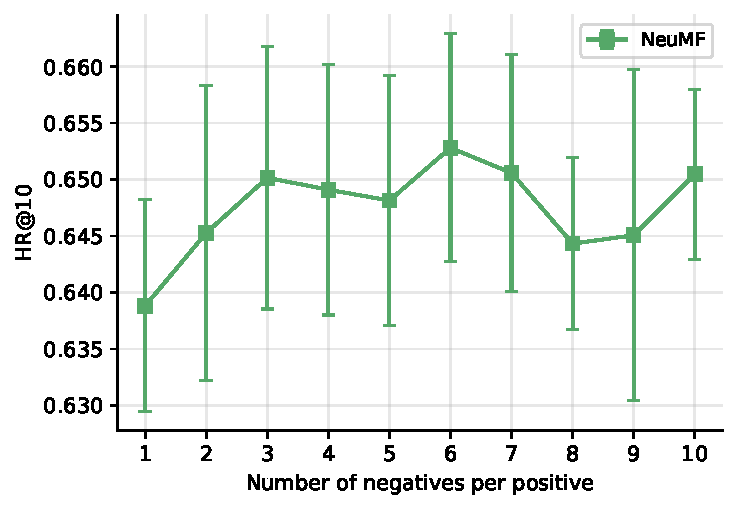
\includegraphics[width=\linewidth]{fig_task07_hr_vs_negatives.pdf}
    \caption{HR@10}
  \end{subfigure}\hfill
  \begin{subfigure}{0.49\linewidth}
    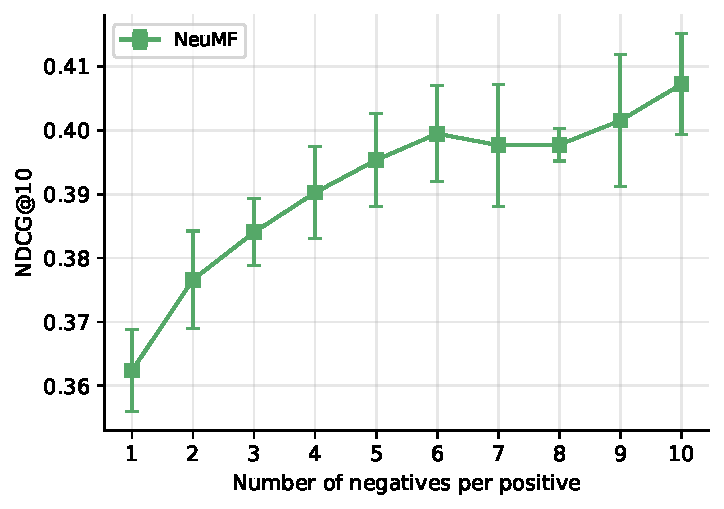
\includegraphics[width=\linewidth]{fig_task08_ndcg_vs_negatives.pdf}
    \caption{NDCG@10}
  \end{subfigure}
  \caption{Effect of the number of negative samples per positive
           interaction on NeuMF. HR@10 saturates after $\sim 3$ negatives;
           NDCG@10 keeps improving up to 10.}
  \label{fig:task07_08}
\end{figure}

% =====================================================================
\section{Non-negative matrix factorisation (Tasks 9 \& 10)}
% =====================================================================

We build a binary user$\times$item interaction matrix
$R \in \{0,1\}^{943 \times 1682}$ from the training positives only and
factor it with \texttt{sklearn.decomposition.NMF} into $R \approx W H$,
where $W \in \mathbb{R}_{\ge 0}^{943 \times k}$ and
$H \in \mathbb{R}_{\ge 0}^{k \times 1682}$. The reconstructed matrix
$\hat{R} = W H$ gives a score $\hat{R}_{ui}$ for every user--item pair,
which we then feed into exactly the same leave-one-out evaluation
protocol as NeuMF (rank the held-out positive against the same 99
sampled negatives). The NMF model has
$k \cdot (|U| + |I|) = 2{,}625 k$ free parameters (the $W$ and $H$
matrices; we do not count transient internal state of the ALS iterations).

\paragraph{NDCG@10 vs.\ $k$ (Task 9).}
Table~\ref{tab:task09_10} and Figure~\ref{fig:task09_10}(a) show that
NDCG@10 rises steeply between $k=1$ and $k=6$
($0.190 \to 0.324$), then more slowly, plateauing around
$k=16$--$26$ at $\sim 0.363$--$0.368$. The best mean NDCG@10 is at
$k=26$ ($0.368 \pm 0.003$), which we adopt as the ``best NMF setting''
for the rest of the report. The standard deviations are very small at
small $k$ (essentially zero for $k \in \{1, 6\}$, where the NNDSVD
initialisation in scikit-learn is deterministic and the global optimum
of a rank-1/6 factorisation is well defined), and grow modestly as $k$
increases.

\paragraph{Parameter count vs.\ $k$ (Task 10).}
Figure~\ref{fig:task09_10}(b) shows the parameter count of NMF grows
exactly linearly with $k$ (it is $(943 + 1682)k$), from $2{,}625$ at
$k=1$ to $68{,}250$ at $k=26$. In contrast to NeuMF --- whose parameter
count is dominated by the four fixed-size embedding tables and barely
moves with MLP depth --- NMF's parameter budget scales freely with the
modelling capacity.

\begin{table}[H]
  \centering
  \caption{NMF on MovieLens-100K: HR@10, NDCG@10 and parameter count
           vs.\ the number of latent factors $k$ (mean $\pm$ std,
           10 seeds).}
  \label{tab:task09_10}
  \inputtab{tab_task09_10_nmf}
\end{table}

\begin{figure}[H]
  \centering
  \begin{subfigure}{0.49\linewidth}
    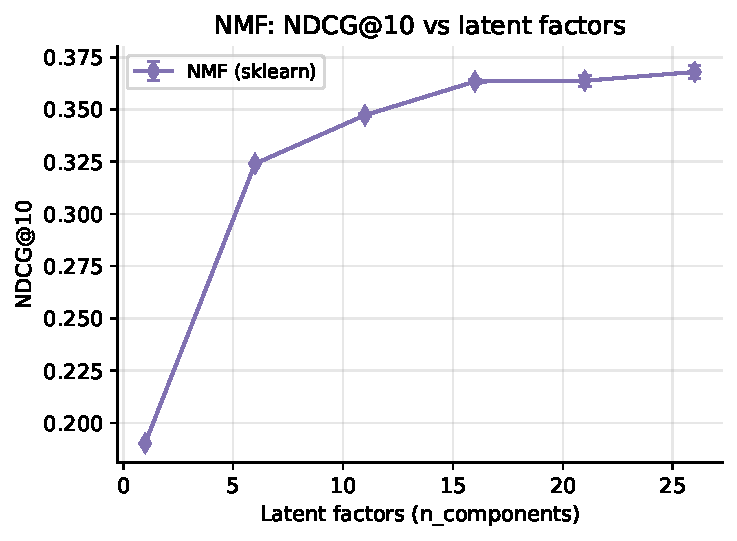
\includegraphics[width=\linewidth]{fig_task09_nmf_ndcg.pdf}
    \caption{Task 9: NDCG@10 vs.\ $k$}
  \end{subfigure}\hfill
  \begin{subfigure}{0.49\linewidth}
    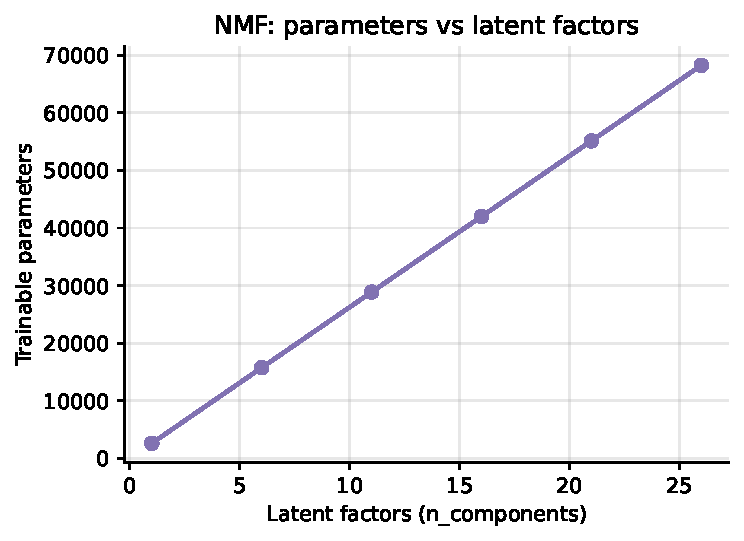
\includegraphics[width=\linewidth]{fig_task10_nmf_params.pdf}
    \caption{Task 10: parameter count vs.\ $k$}
  \end{subfigure}
  \caption{NMF sweep over the number of latent factors,
           $k \in \{1, 6, 11, 16, 21, 26\}$.}
  \label{fig:task09_10}
\end{figure}

% =====================================================================
\section{NeuMF vs.\ NMF comparison (Task 11)}
% =====================================================================

Table~\ref{tab:task11} and Figure~\ref{fig:task11} compare the best NeuMF
(3 MLP layers, no pretraining) with the best NMF ($k=26$). NeuMF wins on
both recommendation metrics: HR@10 is $0.649 \pm 0.011$ vs.\
$0.635 \pm 0.004$ for NMF (a relative improvement of $\sim\!2.2\,\%$),
and NDCG@10 is $0.390 \pm 0.007$ vs.\ $0.368 \pm 0.003$
($\sim\!6.1\,\%$ relative improvement). NeuMF's lead is more pronounced
on NDCG@10 than on HR@10, which is consistent with the observations in
Sections~4 and 6: NeuMF is especially good at pushing the correct item
towards the top of the ranked list, and NDCG is the metric that most
rewards that behaviour.

The comparison is less favourable to NeuMF once parameter count is
considered: NeuMF uses $107{,}761$ parameters against NMF's $68{,}250$,
a $57.9\,\%$ increase. On a per-parameter basis, NMF is actually a very
strong baseline on MovieLens-100K --- the small size of the dataset
plays to the strengths of matrix factorisation, which has no
under-parameterisation issues on a $943 \times 1682$ matrix with 26
latent factors. This observation motivates the knowledge-distillation
experiments of the next section, which show that NeuMF's performance
can be preserved with \emph{fewer} parameters than NMF uses.

\begin{table}[H]
  \centering
  \caption{Head-to-head comparison of NeuMF and NMF at their best
           respective settings (mean $\pm$ std, 10 seeds).}
  \label{tab:task11}
  \inputtab{tab_task11_compare}
\end{table}

\begin{figure}[H]
  \centering
  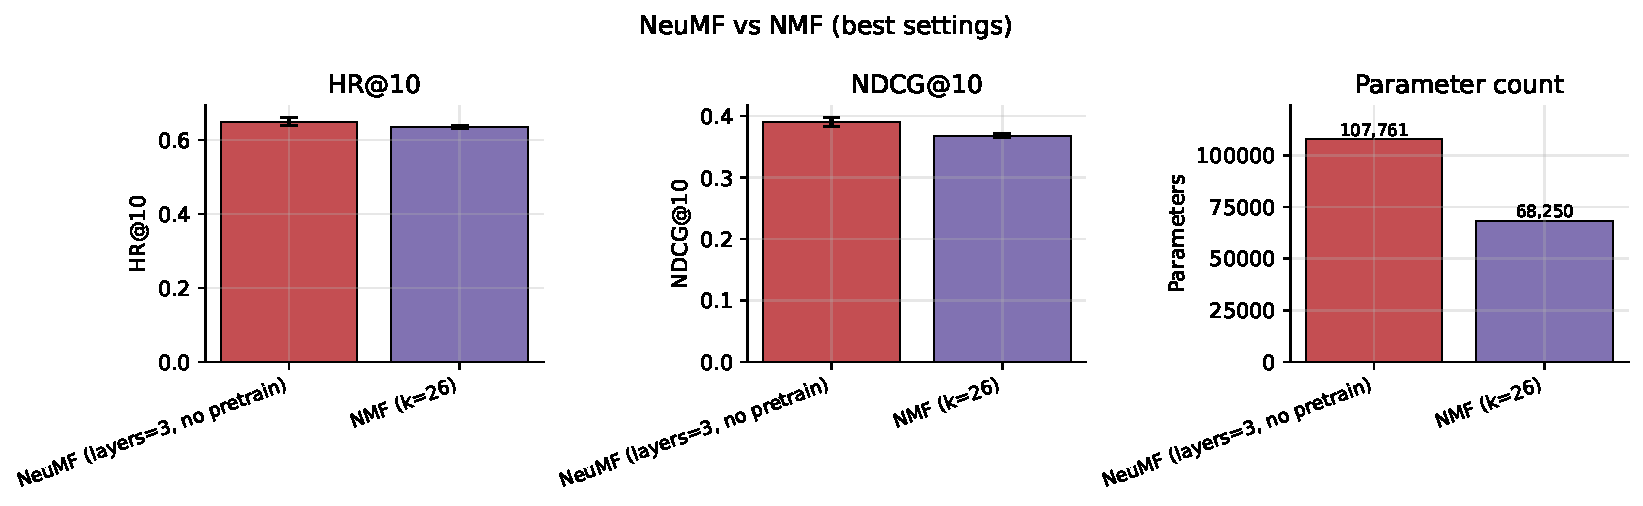
\includegraphics[width=0.96\linewidth]{fig_task11_compare.pdf}
  \caption{Best NeuMF (3 layers, no pretraining) vs.\ best NMF ($k=26$)
           on HR@10, NDCG@10, and parameter count.}
  \label{fig:task11}
\end{figure}

% =====================================================================
\section{Knowledge distillation (Task 12)}
% =====================================================================

We take the best NeuMF from the previous experiments as the teacher
($107{,}761$ parameters) and train three smaller NeuMF students, all
with the same reduced architecture
(\texttt{gmf\_embed\_dim}=4, \texttt{mlp\_embed\_dim}=16, 2~MLP layers,
giving $53{,}177$ parameters --- a 50.7\,\% reduction). The three
students differ only in the distillation objective, following the
survey of Gou et al.~\cite{gou2021kd}:

\begin{enumerate}
  \item \textbf{Response-based KD}~\cite{hinton2015distilling}:
        binary-cross-entropy between the student's
        temperature-scaled logits and the teacher's
        temperature-scaled soft probabilities. We combine with the
        standard hard-label BCE via an $\alpha$-weighted sum
        ($\alpha = 0.5$, $T = 2$) and scale the soft term by $T^2$
        to preserve gradient magnitudes as in the original paper.
  \item \textbf{Feature-based KD / FitNets}~\cite{romero2014fitnets}:
        MSE between the student's fused representation (concatenation
        of the GMF element-wise product and the MLP last hidden layer)
        and the teacher's fused representation. Because the two fused
        vectors have different dimensions ($20$ for the student,
        $72$ for the teacher), we learn a linear projection
        $P \in \mathbb{R}^{72 \times 20}$ of the student representation
        to the teacher's dimension. Total loss is
        hard-BCE $+ \beta \cdot \mathrm{MSE}$ with $\beta = 1$.
  \item \textbf{Relation-based KD / RKD}~\cite{park2019rkd}: within each
        mini-batch we compute the pairwise $L_2$-distance matrices of
        the (projected) student and teacher fused features, normalise
        each by its mean as in the original paper, and minimise the
        smooth-$L_1$ (Huber) loss between them. Total loss is
        hard-BCE $+ \gamma \cdot \mathrm{RKD}$ with $\gamma = 1$.
\end{enumerate}

Table~\ref{tab:task12} and Figure~\ref{fig:task12} summarise the results.
Three findings stand out:

\begin{itemize}
  \item \textbf{Response-based KD matches and even slightly exceeds the
        teacher's HR@10} ($0.655 \pm 0.010$ vs.\ $0.649 \pm 0.011$) while
        using \textbf{50.7\,\% fewer parameters}. NDCG@10 drops modestly
        from $0.390$ to $0.378$ ($-3\,\%$ relative). This is the textbook
        outcome of knowledge distillation: the student inherits the
        teacher's ranking behaviour through the soft targets without
        needing the full architectural capacity to rediscover it from
        hard labels alone.
  \item \textbf{Relation-based KD retains most of the teacher's
        performance} (HR@10 $0.630$, NDCG@10 $0.364$), but is a few
        points behind response-based KD. Preserving pairwise-distance
        relations in representation space is evidently a weaker signal
        than directly copying the output distribution for this task.
  \item \textbf{Feature-based KD underperforms} (HR@10 $0.582$,
        NDCG@10 $0.330$, $\sim\!10\,\%$ and $\sim\!15\,\%$ relative
        drops respectively). Forcing the student's 20-dimensional fused
        representation to linearly project onto the teacher's
        72-dimensional one is a strong constraint that may be
        over-regularising the student and diverting gradient budget
        away from the actual ranking objective. FitNets-style hint
        losses typically benefit from careful layer selection and
        $\beta$-tuning, neither of which we explored here.
\end{itemize}

The practical takeaway is that on MovieLens-100K a NeuMF student with
only $53{,}177$ parameters --- \emph{fewer than the 68{,}250 used by the
best NMF baseline} --- can preserve the teacher's HR@10 when trained with
response-based distillation. In other words, the parameter-count
disadvantage of NeuMF observed in Section~7 is largely closeable through
KD.

\begin{table}[H]
  \centering
  \caption{Teacher NeuMF vs.\ three distilled students with the same
           smaller architecture (mean $\pm$ std, 10 seeds). All three
           students have the same parameter count; they differ only in
           the distillation loss used during training.}
  \label{tab:task12}
  \inputtab{tab_task12_kd}
\end{table}

\begin{figure}[H]
  \centering
  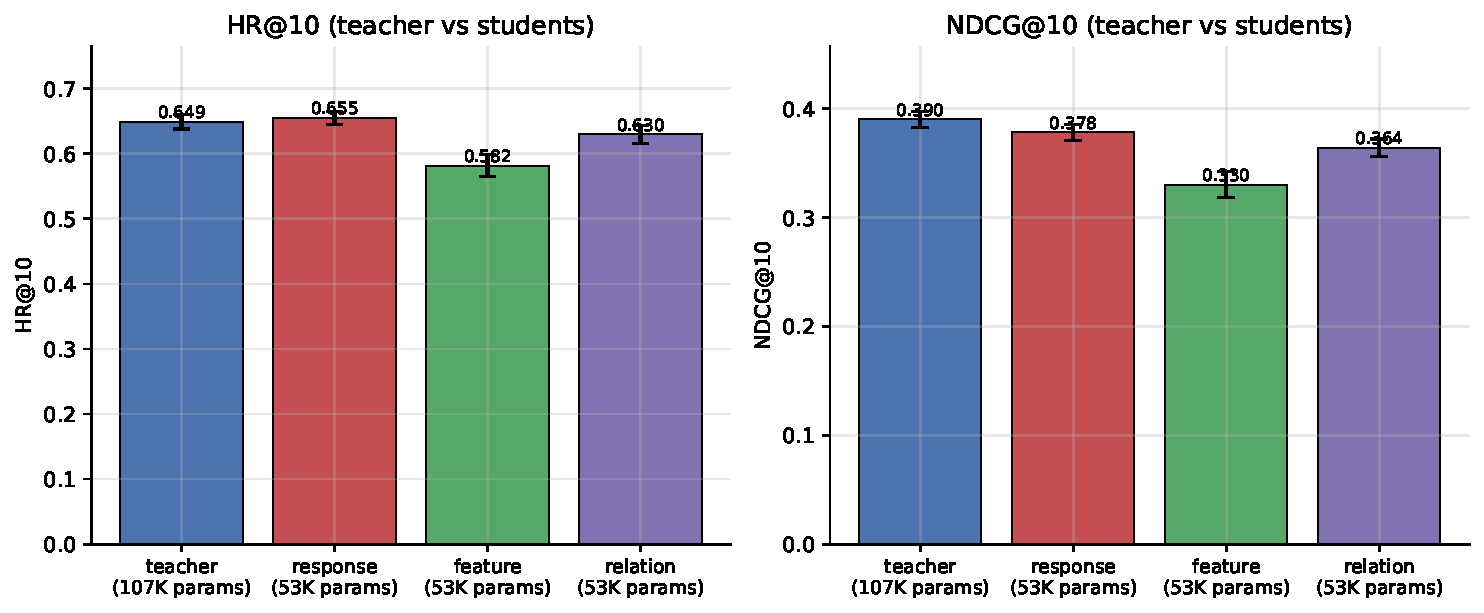
\includegraphics[width=0.98\linewidth]{fig_task12_kd.pdf}
  \caption{HR@10 and NDCG@10 of the teacher NeuMF ($107{,}761$ parameters)
           and three distilled students with identical reduced
           architecture ($53{,}177$ parameters each). Error bars are
           $\pm 1$ std over 10 seeds.}
  \label{fig:task12}
\end{figure}

% =====================================================================
\section*{Reproducibility}
% =====================================================================

All source code, experimental scripts, figures, tables and a Kaggle
runner notebook are available at
\url{https://github.com/mavroul1s/ncf-assignment}. The complete pipeline
(10 seeds, 20 epochs per run, all 12 tasks) reproduces in roughly
3--4 hours on a single NVIDIA Tesla T4 GPU by running the provided
Kaggle notebook; outputs are written to \texttt{results/}, which is
consumed directly by this report.

% =====================================================================
\begin{thebibliography}{9}
% =====================================================================

\bibitem{he2017ncf}
X.~He, L.~Liao, H.~Zhang, L.~Nie, X.~Hu, and T.-S.\ Chua.
\newblock {\em Neural Collaborative Filtering}.
\newblock In WWW, 2017. \href{https://arxiv.org/abs/1708.05031}{arXiv:1708.05031}.

\bibitem{gou2021kd}
J.~Gou, B.~Yu, S.~J.\ Maybank, and D.~Tao.
\newblock {\em Knowledge Distillation: A Survey}.
\newblock International Journal of Computer Vision, 2021.
\href{https://arxiv.org/abs/2006.05525}{arXiv:2006.05525}.

\bibitem{hinton2015distilling}
G.~Hinton, O.~Vinyals, and J.~Dean.
\newblock {\em Distilling the Knowledge in a Neural Network}.
\newblock NeurIPS Deep Learning Workshop, 2015.
\href{https://arxiv.org/abs/1503.02531}{arXiv:1503.02531}.

\bibitem{romero2014fitnets}
A.~Romero, N.~Ballas, S.~E.\ Kahou, A.~Chassang, C.~Gatta, and Y.~Bengio.
\newblock {\em FitNets: Hints for Thin Deep Nets}.
\newblock In ICLR, 2015.
\href{https://arxiv.org/abs/1412.6550}{arXiv:1412.6550}.

\bibitem{park2019rkd}
W.~Park, D.~Kim, Y.~Lu, and M.~Cho.
\newblock {\em Relational Knowledge Distillation}.
\newblock In CVPR, 2019.
\href{https://arxiv.org/abs/1904.05068}{arXiv:1904.05068}.

\end{thebibliography}

\end{document}